\documentclass{article}
\usepackage{amsmath,amssymb}%添加数学宏包
\usepackage{graphics,subfigure}
\usepackage{grffile}
\usepackage{CTEX}
\usepackage{parskip}
\newcommand{\displayimage}[2][width=\textwidth]{%
  \begin{figure}[htbp]
    \centering
    \includegraphics[#1]{#2}
  \end{figure}
}

\begin{document}
\title{tcpiplab}
\author{221501029潘泓旭}
\date{221501029@smail.nju.edu.cn}
\maketitle
\noindent
%插入图片
1.我的ID:172.24.38.17,TCP端口:2952\\
2.服务器端口:8080\\
\displayimage{pic2/p1.png}

3.TCP(6)\\
\displayimage{pic2/p2.png}

4.20bytes,有效负载为总长度-报头长度=1341\\
\displayimage{pic2/p3.png}
\newpage
5.没分段,因为Don't fragment是Set,More fragments是Not set,\\fragment offset也为0\\
6.  59195,128\\
\displayimage{pic2/p5.png}

7.相对序列号为151837,绝对序列号为2818240797;根据三次握手,客户端发送SYN请求来建立连接
,我找到发送的第一个请求并且发现我电脑把SYN标为151837从而建立连接,sequence number:2818240797是个随机值,以上是三次握手的第一步\\
\displayimage{pic2/p6.png}

8.381,153158(2818242118)Acknowledge number是前面那个的Next Sequence Number;
意思是服务器收到连接请求并且发送SYN-ACK确认,这是三次握手第二步骤\\
\displayimage{pic2/p7.png}
\newpage
9.  1\\
\displayimage{pic2/p8.png}

10.如表所示;\displayimage{pic2/RTT.png}\\
EstimatedRTT=0.875*EstimatedRTT+0.125*SampleRTT\\
%\displayimage{pic2/p10.png}
%\displayimage{pic2/p11.png}
%\displayimage[height=38pt]{pic2/1.0.png}
%\displayimage{pic2/2.0.png}
\begin{figure}[htbp]
  \centering
  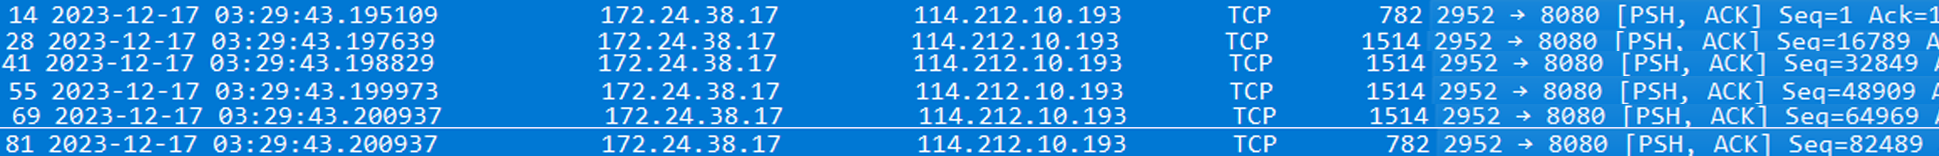
\includegraphics[height=38pt]{pic2/1.0.png}
  \subfigure[发送时间]{
    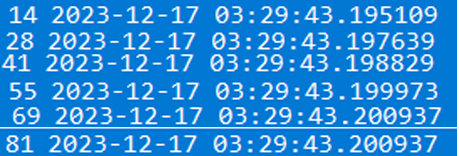
\includegraphics[width=0.45\textwidth]{pic2/1.00.png}
    \label{fig:subfig1}
  }
  \hspace{1cm} % 调整两张图片的间距
  \subfigure[接收时间]{
    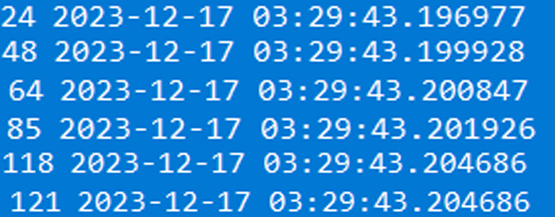
\includegraphics[width=0.4\textwidth]{pic2/2.0.png}
    \label{fig:subfig2}
  }
\end{figure}
\newpage
11.由ACK号,可知长度各为\\
  1)729-1=728\\
  2)18249-729=17520\\
  3)34309-18429=15880\\
  4)50369-34309=16060\\
  5)66429-50369=16060\\
  6)83217-66429=16788\\
\displayimage{pic2/len.png}

12.30720字节(只需看第一个确认(窗口递增)),发送器永远不会因为接收器缓冲区空间不足而被抑制\\
13.没有,为此我检查了TCP数据段的序列号,发现是单调递增的\\
\displayimage[height=200pt]{pic2/seq.png}
\newpage
14.1460,注意到大致都是1460的倍数(16060=1460*11,17520=1460*12)\\
比1460大就可以识别发晚了的情况,我这里就都是这样的(汗颜)\\
15.可以通过第一个TCP数据的序列号和最后一个ACK的序列号计算,此处取六个好了\\
(121-14)/(0.204686-0.195109)=11172.6(字节/秒)
\displayimage[height=300pt]{pic2/v.png}

\end{document}